\chapter{Introduction to Deterministic Methods}
\label{chap:determ_intro}

\epigraphhead[10]{\singlespacing
    \epigraph{
        I love America more than any other country in the world and, exactly for this reason, I insist on the right to criticize her perpetually.
    }
    {James Baldwin}
}

This chapter provides more specific background and introduction to determent radiation transport methods needed before my manuscript chapters.
I discuss the state of the art in deterministic radiation transport on GPUs and the various numerical methods needed to solve the 4 independent variable particle intergro-differential equation implemented in this work.
I also summarize manuscript chapters \ref{chap:therefore_paper} and \ref{chap:smom_paper} including their contributions and relationship to my research questions from section \ref{sec:research_qustions}.

\section{S$_N$ approximation in angle}

There are two major methods of treating the double integral over all angle in Eq. \ref{eq:fullNTE}.
The method of spherical harmonics or P$_{N}$ method which takes angular moments of the transport equation then makes a closure assumption at the N\ths  order.
This work focuses on the S$_N$ or discrete ordinance approximation which turns the Eq. \ref{eq:fullNTE} into a coupled (simultaneous) set of linear partial differential equations in each angular direction using quadrature integration.
It was first formulated by Chandrasekhar to describe radiative heat transfer in stellar media \cite{chandrasekhar1960radiative}.
The S$_N$ approximation was soon applied to neutron transport by Carlson \cite{precise1971carlson}, Lee \cite{discrete1961lee}, and Lathrop \cite{discrete1966lathnrop}.
The method of discrete ordinance was also adapted to general radiative heat transfer by Fiveland \cite{three1988fiveland} and Truelove \cite{discrete1987truelove}.

At this point it becomes necessary to describe the other governing assumptions I use in this work including:
slab geometry (1D-rectilinear coordinates), isotropic scattering and sources, as well as the multi-group assumption in energy distribution.
The methods I develop in this work are not restricted by these assumptions---and future work may explore the methods described here in anisotropic distributions in angle and/or solutions on unstructured meshes---but are made here for simplicity.
In fact, I make specific decisions in this work with the underlying discretization schemes to allow for eventual extension to these regimes.

When applied to Eq.~\eqref{eq:fullNTE} the resulting initialization point is described by
\begin{multline}
    \label{sn_nte_int}
    \frac{1}{v_g} \frac{\partial \psi_{m,g}(x,t)}{\partial t} + \mu_m \frac{\partial \psi_{m,g}(x,t)}{\partial x} + \Sigma_g(x) \psi_{m,g}(x,t)  \\
     = \frac{1}{2} \left( \sum\limits_{g' = 0}^G \Sigma_{s, g'\to g}(x) \sum\limits_{n=1}^N w_n \psi_{n, g'}(x,t) + Q_g(x,t) \right) \;, \\
    \qquad g=1 \ldots G \;, \qquad m=1 \ldots N \;, \qquad t > 0 \;, \qquad x \in [0,X] \;,
\end{multline}
where $\psi$ is the angular flux, $x$ and $t$ are independent continuous variables for 1D space and time respectively, $g$ is the group index, $v$ is velocity, $w$ is an angular quadrature weight, $\mu$ is the angular quadrature ordinate ($\cos(\hat{\Omega}_\theta)$), $m$ is the quadrature index, and $Q$ is the isotropic material source.
In this work I will exclusively use Gauss-Legendre quadrature, but if extended to higher dimensions other quadratures sets would be required to evaluate the double integral over both angular directions (e.g., level-symmetric). 
The initial and boundary conditions are again prescribed angular flux distributions:
\begin{equation*}
    \psi_{m,g}(x,0) = \psi_{m,0}(x), \qquad m=1 \ldots N \;,
\end{equation*}
\begin{equation*}
    \psi_{m,g}(0,t) = \psi_{m,L}(t), \qquad \mu_m >0 \;,
\end{equation*}
\begin{equation*}
    \psi_{m,g}(X,t) = \psi_{m,R}(t), \qquad \mu_m <0 \;.
\end{equation*}
From here additional discretization can be used to turn the continuous functions of angular flux, source, material data, and differential operators into numerical approximations.

\section{Time-Space discretization schemes}

To enable this work in both space and time, discretization schemes are needed to treat the differential operators and continuous functions.
As the goal of the research is for development on heterogeneous architectures, communication to work ratio may become an issue.
Numerical algorithms that require lots of communication back and forth between the host (CPU) and device (GPU) will limit the maximum allowable performance for most GPU accelerators.
To abate this issue higher (second) order discretization schemes can be used to add to the compute work required in every iteration, thus improving the communication to work ratio.

Various classes of spatial discretizations can be used in radiation transport.
Finite difference, finite element, and finite volume methods are all often employed with the most common in radiation transport being Diamond-Differencing $\mathcal{O}(2)$.
Diamond-Difference is popular as it is the only second order space discretization that uses a single interior (cell-averaged) degree of freedom; however it only works on orthogonal grids.
%Intended future investigation of the scheme in this research are into non-uniform meshes.
To allow future work to more readily extend the algorithms described here to unstructured grids I make specific decisions about a discritization scheme---in other words, not Diamond-Differencing.
Instead I use a finite volume scheme specifically designed for use on unstructured grids called corner-balance, which was originally developed by Adams~\cite{adams_subcell_1997}.
It is a finite volume method thus it enforces conservation within subcell volumes in a spatial cell.
Simple corner balance was determined to be sufficient as it is higher $\mathcal{O}(2)$ order.
%Simple corner blance is not acrurate in the thin-limit however a slight alteration to it 
Simple corner balance is equivalent to the lumped-linear discontinuous finite element method in 1D.
This spatial discritization is similar to what has previously been implemented in both iterative algorithms explored in this work \ref{sec:syn_acc}.

%Solving the transport equation with deterministic methods typically involves iterative schemes to converge the scattering source and transport operators (this is discussed more in section \ref{sec:intro_itterative-scheme}).
To treat the continuous operators in time, implicit time marching schemes are often used to time step as they have desirable stability properties.
Specifically, implicit (backward) Euler $\mathcal{O}(1)$ or Crank-Nicolson $\mathcal{O}(2)$ are the most often employed.
%These schemes are advantageous as they often act like a wrapper around a steady state deterministic transport solver with few changes needed to implement.
While Crank-Nicolson is second order accurate it is not robust and can produce negative solutions and spurious osculations.
Time dependent version of the multiple balance approach was derived by Variansyah, Larsen, and Martin~\cite{variansyah_robust_2021, ilham_phd} to be a robust, higher (second) order time discretization scheme.
The multiple-balance balance methods was originally developed as a space discretization scheme.

The full space-time-energy-angle discritization scheme is derived in chapter \ref{chap:therefore_paper} and is explicitly shown in Equations \eqref{eq:scatter_mg} and \eqref{eq:fullOCI_mg}.

\section{Iterative Methods}

The linear system of equations formed by the space-energy-time-angle discritization scheme described in the previous sections can be posed as
\begin{equation}
\label{eq:introaxb}
    \bm{A}x=b \; ,
\end{equation}
which may be solved directly (e.g., LU decomposition with pivoting) or iteratively (e.g. Jacobi or Gauss--Seidel iterations).
The dimensions of these problems is \emph{huge} and sparse, going by the number of:
\begin{itemize}
    \item angles in quadrature: \num{10}--\num{100};
    \item energy groups: \num{1}--\num{100};
    \item sub-cell discretizations: 4; and
    \item spatial cells: which can be hundreds upto millions for 1D problems.
\end{itemize}
This is the impact of the \emph{curse of dimensionality} and is only further compounded when moving to higher spatial dimensions. 
So direct simulations are often prohibitively memory and computationally expensive.
Most often these systems are solved with some kind of iterative scheme.

To solve the discritization system iteratively, a fixed point (or Richardson) iteration is often used.
They are broad class of iterative methods where \emph{old} information (from the immediately previous iteration) is used to forum a new right hand side which in turn is resolved for a new guess
Thus the direct formulation in Eq. \eqref{eq:introaxb} becomes
\begin{equation}
    \bm{A}x^{l+1} = b x^{l}
\end{equation}
where $l$ is the iteration counter.
The iteration will continue until the quantity of interest stops changing between iterations when we say the scheme has \emph{converged}.

The process of separating components of the dependent variable to either side of an equation, letting one lag, and solving for an update is called \emph{operator splitting}.
The specifics of a given operator splitting will determine the organization of the linear systems in $A$ and $b$ which in turn will determine how they can be efficiently solved within each iteration and what tools can be used to implement those solvers.
The operator splitting will also impact how many iterations it will take to reach convergence.

For high fidelity problems these systems are still massive and require their solution to be computed in parallel to 




\subsection{Source-iteration}
\label{sec:intro_itterative-scheme}

Due to the curse of dimentionality the linear system
The transport equation requires some kind of iterative scheme to converge the linkage between scattering source and transport operators.
The source iteration (SI) method is commonly used to do this, often accompanied by preconditioners or synthetic accelerators, where the contribution to the solution from the scattering source (summation in the RHS of Eq.~\eqref{sn_nte_int}) is allowed to lag, while the angular flux is solved in every ordinate via transport sweeps through the spatial domain \cite{adams_subcell_1997}.
SI sweeps in Cartesian geometries are readily parallelized over the number of angles, as the source term is known from the previous iteration, allowing the angular flux in each ordinate to be computed independently. 
While any parallelization is a boon to performance, a scheme that is embarrassingly parallel over the dimension with the greatest number of degrees of freedom---space---may be advantageous.
In a single spatial dimension SI is \textit{annoying serial} in space and cannot be parallelized.

In higher spatial dimensions, many S$_N$ production codes that implement SI use some kind of wavefront marching parallel algorithm also known as a Kockh-Baker-Alcouff scheme \cite{baker_kba_2017, colomer_parallel_2013} also called "full parallel sweeps" in literature.
In this scheme a sweep begins in a spatial location where all cell dependencies are known from boundary information (e.g., a corner).
From there on a hypothetical 2D grid, the two nearest neighbor cells are computed independently, potentially in parallel; the next step would be 4 cells.
This diagonally expanding wavefront continues to march and is able to better parallelize as many cells spatially as possible eventually saturating the number of work threads if the problem is large enough.
%On CPUs this has been shown to be performant but this changing amount of work is not optimal on GPUs where.
%Performance evaluations of production codes that implement KBA on GPUs is sparse in literature and when avaliable is from proxy-apps.
%Ardra has such a proxy app 
%KBA algorithms are also tricky to efficiently implement in domain decomposed where wave front propagation between boundaries can be tricky.
%While this work is concerned with 1 spatial dimension when analyzing the state of the art it is important to consider that this is done.

%This has proven successful in modern transport applications on CPUs 
%(e.g., PARTISN, which implements the Koch--Baker--Alcouffe or KBA algorithm). 
%The state of the art in deterministic S$_N$ radiation transport is multi-group in energy distribution, diamond differencing first order space discretizations or other FEM FVM schemes on unstructured meshes, backward euler time stepping, domain decomposition via parallel block Jacobi, wave front marching schemes like KBA in higher spatial dimensions within a subdomain, and source iterations with diffusion synthetic acceleration (DSA) and potentially accompanied by GMRES solvers. Some examples of production codes that implement this are Partisn, Ardra, Minerate, Capsaicin, Denovo, Silver Fir, etc.
%Here again this is included as a
%Each one of these points becomes more difficult to implement due to angle-parallel SI with KBA, for example domain decomposition 

%Published literature on what schemes are implemented, how and their performance on GPU accelerators is sparse.
%Most of my understanding of what is currently used comes from conversations held at conferences with the developers of the codes themselves.
%One place I was able to find performance data on is a mini-app called Kripky \cite{kunen_kripke_2015}.
%Kripke is the publicly distributed version of Ardra that has performance data available.
%Roofline anylisys of Kripke has been published for performance on an AMD MI200 GPUs \cite{wolfe2022roofline}. 
%Specific k
%We conject that this is due to the nonlinear work load a wavefront marching schemes incurred. 


\subsection{One cell inversion-iteration}

% Intro to OCI and previous work including warsaw 

One Cell Inversions (OCI) (also called cell-wise parallel block Jacobi) is an alternative to SI where all angular fluxes in all ordinates and groups within a cell are computed in a single linear algebra step.
It assumes that the angular fluxes incident on the surfaces of the cell are known from a previous iteration.
OCI allows for parallelizing over the number of cells as each cell is solved independently of the others in a parallel.

Rosa Warsaw and Perks (2013) \cite{rosa_cellwise_2013} previously investigated OCI as a potentially superior iterative scheme over SI on vectroized heterogeneous architectures.
They supposed that because of the parallelism over the dominant domain, inherit data locality, ability to take advantage of LAPACK type libraries, and highly floppy operations present in an OCI type algorithm, it might out-perform an SI based implementation in wall clock runtime.
The study was conducted on the state of the art (at the) time RoadRunner super computer at Los Alamos National Lab and took advantage of its 64 bit PowerXCell vectorized accelerator---a precursor to GPGPUs seen in HPCs today.
Rosa et al. implemented OCI in a 2D, multi-group, steady state, code using bilinear discontinuous finite element method to discretize space \cite{tsa_2d2007rosa}, a multi-group scheme in energy distribution, and parallel block Jacobi and Gauss-Sidle iterations.

The authors concluded that the acceleration seen per-iteration in OCI was not enough to make up for the decay in convergence rate that OCI incurs.
As there is no communication of information between cells within an iteration (also called a-synchronicity), OCI can require more iterations to converge to a solution for some of problems. 
Specifically, as cellular optical thickness goes down, OCI's relative performance degrades with a spectral radius not bounded by one independent of scattering ratio.
Figure~\ref{fig:specrad} illustrates this behavior, showing the spectral radii of the two iteration schemes as a function of cell thickness (in mean free path) and the scattering ratio.
These values were computed numerically from an infinite medium problem (via reflecting boundaries) using steady-state calculations in S$_4$. 
The smaller the spectral radius, the faster a method is converging.
The spectral radius for SI depends linearly on the scattering ratio, and for problems that are many mean free paths in size, it is nearly independent of cell optical thickness. 
The spectral radius of OCI decreases substantially as the optical thickness of the cells increases.
\begin{figure}[!htb]
    \centering
    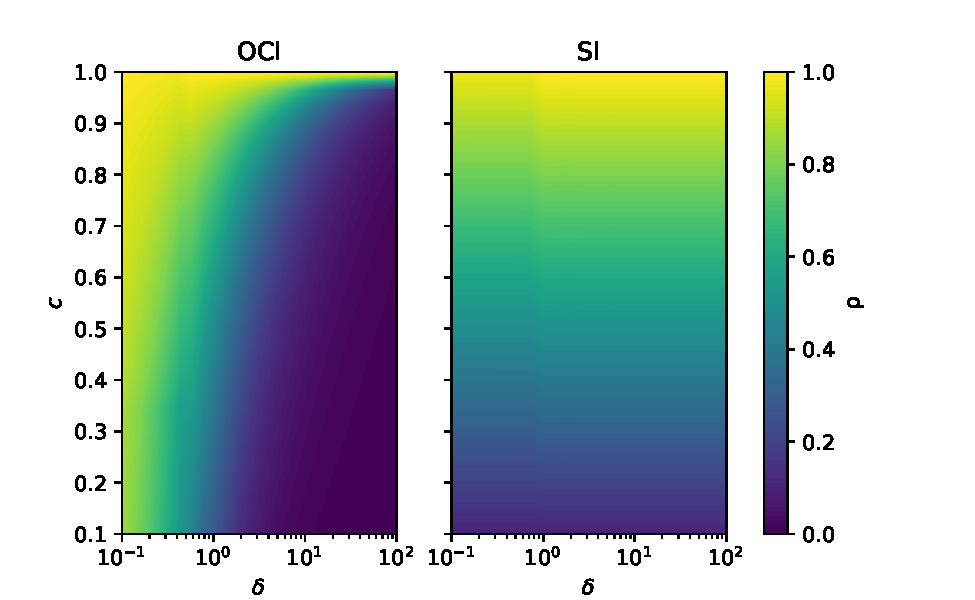
\includegraphics[width=\textwidth]{figures/therefore_figs/ss_specrads.pdf}
    \caption{Spectral radii ($\boldsymbol{\rho}$) of OCI (left) and SI (middle) and the ratio between the two (right), where $\boldsymbol{\Sigma}$ is the total cross section, $\boldsymbol{\Delta x}$ is the cell width, and $\boldsymbol{\Sigma_s}$ is the scattering cross section}
    \label{fig:specrad}
  \end{figure}
Rosa et al. also suggested that future developments in GPU accelerators might overcome this convergence rate decay for problems of interest.
The idea there as that even though more iterations will be required to converge a solution those iterations will be able to be done sufficiently faster (in wall-clock-runtime) to mean a solution is computed faster (again in wall clock runtime) then source iterations.

Other investigations have explored OCI as an acceleration scheme for SI \cite{anistratov_iterative_2015, hoagland_hybrid_2021}. %and a solution to the integral transport matrix method \cite{raffi2108pidotscom} and in the inexact parallel Jacobi scheme.
Previous investigations of OCI as an iterative scheme have been limited to steady state computations.

% potential transient effects in the thin limit 
%When solving discrete ordnance problems for transient systems many codes have implemented Crank-Nicholson or backward Euler time stepping.
%These schemes are non-intrusive often looking like an additional time marching loop around the already implemented transport infrastructure.
Regardless of the time stepping method an OCI iterative algorithm might come with some added befits when used in a transient scheme.
Returning to OCI's spectral radius shown at left in Fig.~\ref{fig:specrad}, since both dimensions are governed by relationships with the cross section of the cell ($\Sigma$), altering that value will impact convergence behavior. 
As the scattering ratio decreases, both iterative algorithms require fewer iterations to converge.
However, the spectral radius of OCI also decreases with increasing optical thickness, \textit{which is an added benefit}.
When solving optically thick and highly scattering problems, small increases in $\Sigma$ may drastically improve the relative performance of OCI in comparison with SI.
%Physically this can be understood as single particles living in single cells for many more iterations.
Time step and cellular optical thickness are inversely proportional to each other, meaning a smaller time step will yield a larger effective total cross section, thus theoretically improving the spectral radius.
This behavior is not expected to happen in source iterations as SI does not directly depend on cellular optical thickness---behaving linearly in that dimension for all but the most thick problems.

\subsection{Preconditinoers and Synthetic acceleration}

\label{sec:syn_acc}
% acceleration schemes for SI
In order to converge iterative schemes faster many synthetic acceleration techniques have been explored and implemented over the years \cite{adams_fast_2002}.
The most common approach used in conjunction with source iterations is diffusion synthetic acceleration (DSA)\cite{adams_fast_2002}.
The slow convergence of SI in the diffusive limit can be physically understood as there is no linking between angles within an iteration and a diffusive problem is a coupling of angles.
DSA adds a mid-step correction term based off of a cheap to compute diffusion approximation.
%Other synthetic acceleration techniques include Boundary projection acceleration \cite{adams_fast_2002}. %find more

% acceleration schemes for OCI
Previous work has also gone into exploring synthetic acceleration techniques for one cell inversions \cite{ kim_coarse_2000}.
OCI is slow to converge in the thin limit due to the a-synchronicity of the scheme (lagging cell-wise boundary fluxes) \cite{hoagland_hybrid_2021}.
The spectral radius will increase unbounded in the thin limit, regardless of scattering ratio \cite{rosa_cellwise_2013}.
Rosa and Warsa (2009) investigated using transport synthetic acceleration (TSA) as a low order synthetic accelerator, performing a Fourier analysis \cite{tsa2009rosa, tsa_slab2006rosa, tsa_2d2007rosa}.
TSA uses a low order transport sweep with potentially fewer angles and a smaller scattering ratio (often controlled by the user by term $\beta \in [0,1]$) to inform the error correction~\cite{tsa1997gilles}.
In effect, TSA is a less expensive transport sweep that re-couples angles together, which is annoyingly parallel in space and may have significant performance impacts to an OCI scheme.
Rosa and Warsa say as much when they suggest an algorithm where a mesh sweep is only used if convergence hasn't been achieved after a given number of iterations \cite{tsa2009rosa}.
%TSA
%While they suggest future work to implement, no published results of an OCI+TSA scheme.

% gmres
Both SI and OCI are forms of a fixed-point (or Richardson) iteration that use different operator splittings.
In a fixed-point iteration an initial guess of the angular or scalar flux is supplied as a known to the solver which in turn returns an angular or scalar flux (see section \ref{sec:syn_acc}).
This becomes the new guess and this iterative process continues until the relative error between the guess and the output falls below a given tolerance \cite{lewis_computational_1984}.
Krylov methods work by keeping copies of the guess for a given number of previous iterates, compute residuals and ensure the next guess is orthogonal to the previous ones\cite{gmres1996kelley, patton_gmres_2002}.
The generalized minimal residual (GMRES) method specifically, has been shown to make DSA schemes that perform relatively poorly, work well \cite{kylov2004warsa, subspace2004warsa}.


\subsection{The Spectral Radius and Eigen Values}


\section{Summary of Part and relation to research questions}


Chapter \ref{chap:therefore_paper}
In this work, we analyze how the convergence rate of an OCI scheme behaves when used for time-dependent neutron transport computations.
We derive a second-order space-time discretization method from the simple corner balance and multiple balance time discretization schemes and show via Fourier analysis that it is unconditionally stable through time.
Then, we derive and numerically solve the Fourier systems for both OCI and SI splittings of our discretization, showing that small mean-free times improve the spectral radius of OCI more than SI, and that spectral radius for OCI tends to zero as mean free time gets smaller.
We extend both solvers to be energy dependent (using the multi-group assumption) and implement on an AMD MI250X using vendor-supplied batched LAPACK solvers.
Smaller time steps improve the relative performance of OCI over SI, and, even when OCI requires more iterations to converge a problem, those iterations can be done much faster on a GPU.
This leads to OCI performing better overall than SI on GPUs.

In this work I limit to a single spatial dimension.
This because the problems we are tying to solve (balancing parallelism, time dependence, convergence rate, and searching preconditioners) is dreadfully difficult.
While the problems I solve are not


Chapter \ref{chap:smom_paper}
Solving the S$_N$ radiation transport equation on modern many cored compute architectures (i.e., GPUs) is challenging.
The most common implemented solution method, the source iteration, requires computational expensive sweeping operations that cannot parallelized in 1D.
While in 2D and 3D sweeps can use full parallel sweeping algorithms these schemes may not perform well on a GPU.
One cell inversion iteration is another class of solvers for the radiation transport equation.
OCI iterations are parallel over spatial cells which has been previously shown to out perform similarly implemented versions of unpreconditioned source iterations on GPUs for some problems.
While OCI is rapidly convergent for optically thick problems spectral radius tends to one in both the optically thin and diffusive limits.
Finding a preconditioner for one cell inversion iterations to support converging in this regime that can be efficiently computed on many-cored architectures motivates this work.
%We have previously shown that for time dependent problems OCI's spectral radius has an added dependence on mean free time and tends to zero as mean free time decreases.
We derive a second moment cellular decomposition method in conjunction with a one-cell inversion iteration in an effort to produce a fully space parallel, rapidly convergent, transport iteration.
The second moment preconditioner derived in this work does not converge to the same solution as unpreconditioned transport solutions suggesting inconsistencies.
Numerical experiments show the second moment preconditioner is rapidly convergent in the diffusive limit but dose not aid convergence in the optically thin limit.


The first publication associated with this work is motivated by the hypothesized additional benefit of OCI in a time dependent code (RQ 3) coupled with the vast improvements in GPU accelerators in the past decade since Rosa et al. \cite{rosa_cellwise_2013} conducted their investigations (RQ 1 and 2).
A rough draft of this first publication is included in Appendix \ref{app:therefore}.
I plan to submit this work before the new year.
The next publication will be an exploration of a synthetic acceleration algorithm to converge OCI in the thin limit (RQ 4).
%Furthermore, as previously mentioned, source iterations are often implemented in production accompanied by some kind of synthetic-acceleration scheme or other preconditioner to converge it's slowest converging mode (the diffusive limit).
%OCI has never been implemented with a prevonditon

To recast the neutron radiation transport equation (Eq.~\eqref{eq:fullNTE}) into a form solvable on digital computers, continuous functions of space, time, angle, and energy must be discretized.
An iterative scheme is also required for memory and computationally efficient calculations.
In this section I describe the discretizations and their assumptions for the 1D, time-dependent, multi-group solver discussed within this work.
I will also describe the two fixed-point iterative schemes that I implement and discuss gaps in previous work of deterministic iterative solvers.
My work with deterministic schemes can be separated into two categories:
\begin{enumerate}
    \item How to use software engineering libraries to implement work more efficiently (RQ 1); and
    \item Novel methods to converge the solution faster on modern hardware
    \begin{enumerate}
        \item A space-parallel iterative scheme on modern HPC GPUs (RQ2);
        \item How transient behavior impacts convergence of a space-parallel iterative scheme (RQ3); and
        \item How to accelerate the space-parallel iterative scheme to converge faster (RQ4)
    \end{enumerate}
\end{enumerate}

